\input /users/davidmcallester/icloud/tex/SlidePreamble
\input /users/davidmcallester/icloud/tex/preamble
\newcommand{\bayes}{\mathrm{Bayes}}

\begin{document}

{\Huge

  \centerline{\bf TTIC 31230, Fundamentals of Deep Learning}

\bigskip

\centerline{David McAllester, Autumn  2024}

\vfill \vfill

\centerline{\bf Variational Auto-Encoders (VAEs)}

\vfill \vfill

\slide{Fundamental Equations of Deep Learning}

\begin{itemize}
\item Cross Entropy Loss: $\Phi^* = {\color{red} \argmin_\Phi E_{(x,y)\sim \pop}\left[-\ln P_\Phi(y|x)\right]}$.

\vfill
\item GAN: $\gen^* = {\color{red} \argmax_{\gen} \min_{\disc} E_{i \sim \{-1,1\}, y \sim P_i}\left[-\ln P_{\disc}(i|y)\right]}$.

\vfill
\item VAE (including diffusion models)
\begin{eqnarray*}
& & \pri^*,\dec^*,\enc^* \\
\\
& = & {\color{red} \argmin_{\pri,\dec,\enc}\;E_{y \sim \pop,z \sim P_\enc(z|y)}\left[ - \ln \frac{P_\pri(z)P_\dec(y|z)}{P_\enc(z|y)}\right]}
\end{eqnarray*}
\end{itemize}

\slide{VAEs}
A variational autoencoder (VAE) is defined by three parts:

\vfill
\begin{itemize}
\item An encoder distribution $P_\enc(z|y)$.

\vfill
\item A decoder distribution $P_\dec(y|z)$

\vfill
\item A ``prior'' distribution $P_\pri(z)$

\end{itemize}

\vfill
VAE generation uses $P_\pri(z)$ and $P_\dec(y|z)$.

\vfill
VAE training uses the encoder $P_\enc(z|y)$.

\slide{Two Joint Distributions}

A VAE defines two joint distributions on $y$ and $z$, namely $P_\bayes(y,z)$ and $P_\enc(y,z)$ defined by

\vfill
$${\color{red} P_\bayes(y,z) = P_\pri(z)P_\dec(y|z)}$$

\vfill
$${\color{red} P_\enc(y,z) = \pop(y)P_\enc(z|y)}$$

\slide{Training the Bayesian Model}

Fix the encoder arbitrarily and train $P_\bayes$ by cross entropy.

$${\color{red}\bayes^* = \argmin_{\bayes}\;E_{(y,z) \sim P_\enc(y,z)}\left[-\ln P_\bayes(y,z)\right]}$$

\vfill
Under Universality we have that generating $y$ from $P_{\bayes^*}$ now samples $y$ from $\pop$.

\slide{Training the Encoder}

If the Bayes model is not universal then the choice of encoder matters.

{\color{red}
\begin{eqnarray*}
\pop(y) & = & \frac{\pop(y)P_\enc(z|y)}{P_\enc(z|y)} \;=\; \frac{P_\enc(y,z)}{P_\enc(z|y)} \\ \\
\\
H(y) & \leq & E_{(y,z) \sim P_\enc}\left[ - \ln \frac{P_\bayes(y,z)}{P_\enc(z|y)}\right] \\
\\
\\
\enc^* & = & \argmin_\enc\;E_{(y,z) \sim P_\enc}\left[ - \ln \frac{P_\bayes(y,z)}{P_\enc(z|y)}\right]
\end{eqnarray*}
}

\slide{VAEs Evolved from Variational Bayesian Inference}
Here $y$ is the evidence about $z$ under the Bayesian model.

{\color{red}
{\huge
\begin{eqnarray*}
\ln P_{\mathrm{Bayes}}(y) & =  & \ln \frac{P_{\mathrm{Bayes}}(y)P_{\mathrm{Bayes}}(z|y)}{P_{\mathrm{Bayes}}(z|y)} \\
\\
\\
& = & E_{z \sim P_\enc(z|y)} \left[\ln \frac{P_{\bayes}(y,z)}{P_{\mathrm{Bayes}}(z|y)}\right] \\
\\
\\
& \geq & E_{z \sim P_\enc(z|y)}\left[\ln \frac{P_{\bayes(y,z)}}{P_\enc(z|y)}\right] \\
\end{eqnarray*}
}}
Here we have replaced a cross-entropy by an entropy.

\slide{Variational Bayesian Inference}
$y$ is the evidence about $z$ under the Bayesian model.

\vfill
{\color{red}
{\huge
\begin{eqnarray*}
\ln P_{\mathrm{Bayes}}(y) & \geq & E_{z \sim P_\enc(z|y)}\left[\ln \frac{P_\bayes(y,z)}{P_\enc(z|y)}\right]
\end{eqnarray*}
}}



\vfill
This is the {\bf evidence lower bound} or {\bf ELBO}.

\slide{Variational Bayesian Inference}

{\color{red}
{\huge
\begin{eqnarray*}
\ln P_{\mathrm{Bayes}}(y) & =  & \ln \frac{P_{\mathrm{Bayes}}(y)P_{\mathrm{Bayes}}(z|y)}{P_{\mathrm{Bayes}}(z|y)} \\
\\
\\
& \geq & E_{z \sim P_\enc(z|y)}\left[\ln \frac{P_{\bayes(y,z)}}{P_\enc(z|y)}\right] \\
\\
\\
\enc^* & = & \argmin_\enc E_{z \sim P_\enc(z|y)}\left[\ln \frac{P_{\bayes(y,z)}}{P_\enc(z|y)}\right] \;=\; P_\bayes(z|y)
\end{eqnarray*}
}}


\slideplain{Expectation Maximization (EM)}

EM is used when $P_\enc(z|y)$ can be set to $P_\bayes(z|y)$ but
$P_\bayes(y,z)$ is highly restricted and cannot express $P_\enc(y,z)$.

{\huge
\vfill
\begin{eqnarray*}
\mbox{E step:}\;P_\enc^*(z|y) & = & P_\bayes(z|y) \\
\\
\mbox{M step:}\;P_\bayes^{t+1}(y,z) & = & \argmin_\bayes E_{y \sim \train, z \sim P_\bayes^t(z|y)} \left[-\ln P_\bayes(y,z)\right]
\end{eqnarray*}
}

\slide{Difficulties in Training the Encoder}


$$\enc^* = \argmin_{\enc}\;\;E_{y\sim \pop(y),{\color{red} z\sim P_\enc(z|y)}}\;\left[- \ln \frac{P_\bayes(y,z)}{P_\enc(z|y)}\right]$$

\vfill
Gradient descent on the encoder parameters must take into account the fact that we are sampling from the encoder.

\vfill
Training a sampling distribution typically suffers from {\bf mode collapse} (as in GANs).

\vfill
The encoder can collapses to a fixed $z = 0$. $P_\dec(y|z)$ can always just ignore $z$. We are then back to standard cross-entropy loss.
This is called {\bf posterior collapse}.

\slide{Types of VAEs}

In {\bf a Gaussian VAE} the we have $P_\pri(z)$ and $P_\enc(z|y)$ are both Gaussian distributions on $R^d$.
A diffusion model involves a Gaussian VAE at each incremental step of diffusion.

\vfill
{\bf A Vector Quantized VAE} (VQ-VAE) defines $P_\enc(z|y)$ in terms of vector quantization analogous to $K$-means clustering.
VQ-VAEs provide a translation from continuous data, such as images, to token data that can be modeled with a transformer.
This is used in the image understanding abilities of GPT-4o and in autoregressive image generation
which is competative with diffusion image generation.

\vfill
We will first consider Gaussian VAEs and discuss VQ-VAEs later.

\slide{Gaussian VAEs}

As an example take

\begin{eqnarray*}
P_\pri(z) & = & {\cal N}(0,I) \\
\\
P_\enc(z|y) & = & {\cal N}(\hat{z}(y),I) \\
\\
P_\dec(y|z) & = & {\cal N}(\hat{y}(z),I)
\end{eqnarray*}

\vfill
In general we can use arbitrary Gaussians but this example makes the math simple.
\slide{Gaussian VAEs}

{\huge
\begin{eqnarray*}
&  & E_{(y,z) \sim P_\enc}\;\left[- \ln \frac{P_\pri(z)P_\dec(y|z)}{P_\enc(z|y)}\right] \\
\\
\\
& = & E_{y \sim \pop} \left[ KL(P_\enc(z|y),P_\pri(z)) + E_{z \sim P_\enc(z|y)}\left[- \ln P_\dec(y|z)\right]\right] \\
\\
\\
&=& E_{y \sim \pop} \left[\frac{1}{2}||\hat{z}_\enc(y)||^2 + E_\epsilon\left[\frac{1}{2}||y - \hat{y}_\dec(\hat{z}_\enc(y)+\epsilon))||^2\right]\right]
\end{eqnarray*}
}



\slide{Hierarchical VAEs}


\centerline{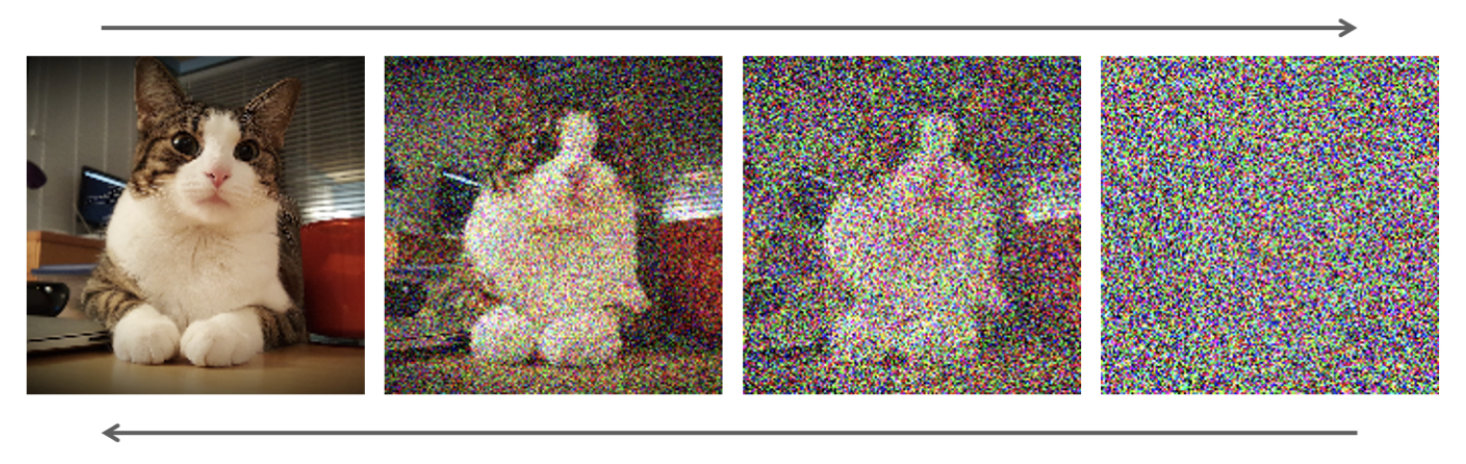
\includegraphics[width = 7in]{\images/DiffSequence}}

\vfill
{\huge
\centerline{{\color{red} [Sally talked to John]} $\stackrel{\rightarrow}{\leftarrow}$ {\color{red} [Sally talked to]}
$\stackrel{\rightarrow}{\leftarrow}$ {\color{red}[Sally talked]} $\stackrel{\rightarrow}{\leftarrow}$ {\color{red}[Sally]} $\stackrel{\rightarrow}{\leftarrow}$ {\color{red} []}}
}

\vfill
\centerline{$y \stackrel{\rightarrow}{\leftarrow} z_1  \stackrel{\rightarrow}{\leftarrow} \cdots \stackrel{\rightarrow}{\leftarrow} z_N$}

\slide{Hierarchical VAEs}
\centerline{$y \stackrel{\rightarrow}{\leftarrow} z_1  \stackrel{\rightarrow}{\leftarrow} \cdots \stackrel{\rightarrow}{\leftarrow} z_N$}

\vfill
{\bf Encoder}: $\pop(y)$, $P_\enc(z_1|y)$, and $P_\enc(z_{\ell+1}|z_\ell)$.


\vfill
{\bf Generator}: $P_\pri(z_N)$, $P_\dec(z_{\ell-1}|z_\ell)$, $P_\dec(y|z_1)$.

\vfill
The encoder and the decoder define distributions $P_\enc(y,\ldots,z_N)$ and $P_\dec(y,\ldots,z_N)$ respectively.


\slide{Hierarchical VAEs}

\centerline{$y \stackrel{\rightarrow}{\leftarrow} z_1  \stackrel{\rightarrow}{\leftarrow} \cdots \stackrel{\rightarrow}{\leftarrow} z_N$}

\vfill
\begin{itemize}
\item autoregressive models

\vfill
\item diffusion models
\end{itemize}


\slide{Hierarchical (or Diffusion) ELBO}

{\Large
\begin{eqnarray*}
H(y) & = & E_\enc\left[- \ln\frac{P_\enc(y)P_\enc(z_1,\ldots,z_N|y)}{P_\enc(z_1,\ldots,z_N|y)}\right]\\
  \\
  \\
  & = & E_\enc\left[ - \ln\frac{P_{\color{red} \enc}(y|z_1)P_{\color{red} \enc}(z_1|z_2)\cdots P_{\color{red} \enc}(z_{N-1}|z_N)P_{\color{red} \enc}(z_N)}
  {P_\enc(z_1|z_2,y)\cdots P_\enc(z_{N-1}|z_N,y)P_\enc(z_N|y)}\right] \\
   \\
   \\
  & {\color{red} \leq} & E_\enc\left[ - \ln\frac{P_{\color{red} \dec}(y|z_1)P_{\color{red} \dec}(z_1|z_2)\cdots P_{\color{red} \dec}(z_{N-1}|z_N)P_{\color{red} \dec}(z_N)}
  {P_\enc(z_1|z_2,y)\cdots P_\enc(z_{N-1}|z_N,y)P_\enc(z_N|y)}\right] \\
\\
\\
 & = & \left\{\begin{array}{l}E_\enc\;[-\ln P_\dec(y|z_1)]
                             \\ \\ + \sum_{i=2}^N  \; E_\enc\; KL(P_\enc(z_{i-1}|z_i,y),\;P_\dec(z_{i-1}|z_i)) \\
                             \\ + E_\enc\; KL(P_\enc(Z_N|y),p_\dec(Z_N))\end{array}\right.
\end{eqnarray*}
}

\slide{END}

\end{document}
